% ============================================================================
%  COMPILE WITH XeLaTeX  (twice, so the point total resolves)
%  Overleaf: Menu -> Compiler -> XeLaTeX
%  Requires: bnhandout.sty and fonts/Kalpurush.ttf in the project
% ============================================================================
\documentclass[11pt]{article}
\usepackage{bnhandout}          % add [nosol] for a student edition

\hauthor[https://jugantordey.github.io]{Jugantor Dey}
\hseries{\textit{Mathematics for the Physics Olympiad}}

\begin{document}

\handouttitle{Chapter 13 : Trigonometry II}

\noindent
শুরু করার আগে ৭ নম্বর অধ্যায় থেকে একক বৃত্ত, radian এবং যোগ ও বিয়োগ সূত্র
চারটি হাতের কাছে নিয়ে বসো; এই গোটা অধ্যায় আসলে ওই চারটি সূত্রকে নানা দিক
থেকে পড়ার গল্প। ৮ নম্বর অধ্যায় থেকে বর্গমূল ও চিহ্ন নিয়ে সাবধানতাটুকু
লাগবে, আর ৪ নম্বর অধ্যায়ের বিপরীত ফাংশনের সংজ্ঞা তৃতীয় অনুচ্ছেদে সরাসরি
কাজে আসবে।

চারটি অনুচ্ছেদের মধ্যে শেষটিই সবচেয়ে বেশি ব্যবহার হবে। পদার্থবিজ্ঞানে যত
আসন্নীকরণ (approximation) করা হয়, তার মধ্যে $\sin\theta \approx \theta$
সম্ভবত সবচেয়ে বেশিবার আসে: দোলক, তরঙ্গ, আলোকবিজ্ঞান, ছোট কম্পন, কৌণিক আকার,
প্রায় সব জায়গায়। তাই ওই অনুচ্ছেদে কেবল সূত্রটা নয়, কতটুকু ভুল হচ্ছে সেটাও
মাপা হবে।

প্রথম দুটি অনুচ্ছেদে নতুন কোনো সত্য নেই, কেবল পুরনো সূত্রগুলোকে অন্যভাবে সাজানো।
সেটাই তাদের শক্তি: একই তথ্য যখন অন্য চেহারায় লেখা যায়, তখন যে সমস্যা আগে অসম্ভব
লাগত সেটাই হঠাৎ সহজ হয়ে যায়। এই অধ্যায়ে মোট \totalpoints\ পয়েন্ট আছে।

\section{গুণফল সূত্র}

৭ নম্বর অধ্যায়ের চারটি সূত্র আবার লিখে নিই, কারণ এই অনুচ্ছেদের সবকিছু
এদের থেকেই আসবে:
\[
  \sin(A \pm B) = \sin A\cos B \pm \cos A \sin B, \qquad
  \cos(A \pm B) = \cos A\cos B \mp \sin A \sin B .
\]

এখন একটা সহজ কিন্তু কার্যকর চাল: এই সূত্রগুলো জোড়ায় জোড়ায় যোগ বা বিয়োগ করলে
এক পাশের গুণফলগুলো কাটাকাটি যায় এবং একটিমাত্র গুণফল টিকে থাকে।

\begin{idea}[গুণফল থেকে যোগফল]
\[
  \sin A\cos B = \tfrac{1}{2}\left[ \sin(A+B) + \sin(A-B) \right] ,
\]
\[
  \cos A\cos B = \tfrac{1}{2}\left[ \cos(A-B) + \cos(A+B) \right] ,
\]
\[
  \sin A\sin B = \tfrac{1}{2}\left[ \cos(A-B) - \cos(A+B) \right] .
\]
\end{idea}

প্রথমটির প্রমাণ: $\sin(A+B)$ ও $\sin(A-B)$ যোগ করলে $\cos A\sin B$ পদ দুটি
চিহ্নে বিপরীত হওয়ায় কাটাকাটি যায় এবং থাকে $2\sin A\cos B$। তৃতীয়টির প্রমাণ:
$\cos(A-B)$ থেকে $\cos(A+B)$ বিয়োগ করলে $\cos A\cos B$ কাটাকাটি যায় এবং থাকে
$2\sin A\sin B$। দ্বিতীয়টিও একইভাবে, কেবল যোগ করে।

উল্টো দিকে যাওয়াটাও একই সূত্রের আরেক পিঠ। উপরের সমীকরণে
$X = A+B$ ও $Y = A-B$ ধরলে $A = \dfrac{X+Y}{2}$ এবং $B = \dfrac{X-Y}{2}$, তাই:

\begin{idea}[যোগফল থেকে গুণফল]
\[
  \sin X + \sin Y = 2\sin\frac{X+Y}{2}\cos\frac{X-Y}{2}, \qquad
  \sin X - \sin Y = 2\cos\frac{X+Y}{2}\sin\frac{X-Y}{2} ,
\]
\[
  \cos X + \cos Y = 2\cos\frac{X+Y}{2}\cos\frac{X-Y}{2}, \qquad
  \cos X - \cos Y = -2\sin\frac{X+Y}{2}\sin\frac{X-Y}{2} .
\]
\end{idea}

আটটি সূত্র মুখস্থ করার কোনো দরকার নেই। একটি কথা মনে রাখলেই চলে: \emph{গুণফল
সূত্রগুলো হলো যোগ সূত্রগুলোকে উল্টো দিক থেকে পড়া}। পরীক্ষার হলে ভুলে গেলে
$\sin(A+B)$ আর $\sin(A-B)$ পাশাপাশি লিখে যোগ করে ফেললেই এক লাইনে বেরিয়ে আসবে।

\begin{example}
$\sin 5x\cos 3x$-কে যোগফল আকারে লেখো, এবং প্রমাণ করো যে
$\cos 5x - \cos x = -2\sin 3x\sin 2x$।
\end{example}

\begin{solbox}
প্রথমটি: $A = 5x$, $B = 3x$ বসিয়ে
\[
  \sin 5x\cos 3x = \tfrac{1}{2}\left[ \sin 8x + \sin 2x \right] .
\]

দ্বিতীয়টি: $X = 5x$, $Y = x$ নিলে $\dfrac{X+Y}{2} = 3x$ এবং
$\dfrac{X-Y}{2} = 2x$, তাই
\[
  \cos 5x - \cos x = -2\sin 3x\sin 2x .
\]
যাচাই করে দেখা ভালো: $x = \pi/6$ বসালে বাম পাশ
$\cos(5\pi/6) - \cos(\pi/6) = -\tfrac{\sqrt{3}}{2} - \tfrac{\sqrt{3}}{2}
= -\sqrt{3}$, আর ডান পাশ
$-2\sin(\pi/2)\sin(\pi/3) = -2 \cdot 1 \cdot \tfrac{\sqrt{3}}{2} = -\sqrt{3}$।
\end{solbox}

\begin{remark}
এই সূত্রগুলো পদার্থবিজ্ঞানে কোথায় লাগে, তার সবচেয়ে সুন্দর উদাহরণ beat। কাছাকাছি
কম্পাঙ্কের দুটি শব্দতরঙ্গ একসঙ্গে বাজলে যোগফল
\[
  \cos\omega_{1}t + \cos\omega_{2}t
  = 2\cos\frac{\omega_{1}-\omega_{2}}{2}t \cdot
    \cos\frac{\omega_{1}+\omega_{2}}{2}t .
\]
ডান পাশটি পড়ো এভাবে: একটি দ্রুত দুলুনি (গড় কম্পাঙ্কের), যার বিস্তার ধীরে ধীরে
ওঠানামা করছে। কানে তাই শোনা যায় একটিমাত্র সুর, যার জোর নিয়মিত বিরতিতে বাড়ে ও
কমে। নিচের ছবিতে ঘন দুলুনিটাই যোগফল, আর ভাঙা রেখা দুটি হলো তার খাম (envelope)।
\end{remark}

\begin{center}
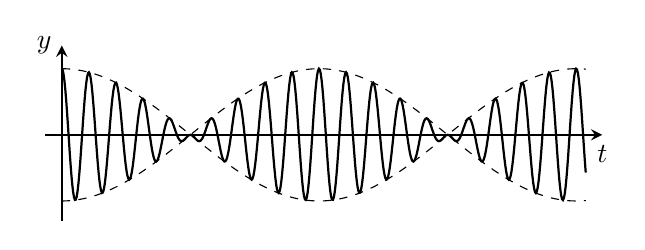
\begin{tikzpicture}[x=0.52cm,y=0.42cm,>=stealth]
  \draw[thick,->] (-0.4,0) -- (13.2,0) node[below] {$t$};
  \draw[thick,->] (0,-2.6) -- (0,2.7) node[left] {$y$};
  \draw[dashed,domain=0:12.8,samples=200,variable=\t] plot ({\t},{2*cos(0.5*\t r)});
  \draw[dashed,domain=0:12.8,samples=200,variable=\t] plot ({\t},{-2*cos(0.5*\t r)});
  \draw[thick,domain=0:12.8,samples=600,variable=\t] plot ({\t},{cos(9*\t r)+cos(10*\t r)});
\end{tikzpicture}
\end{center}

\prob{2} \begin{enumerate}
  \item $2\sin 7x\cos 3x$-কে যোগফল আকারে লেখো।
  \item প্রমাণ করো যে $\sin 3x + \sin x = 2\sin 2x\cos x$।
\end{enumerate}

\begin{sol}
\begin{enumerate}
  \item $2\sin 7x\cos 3x = \sin 10x + \sin 4x$।
  \item $X = 3x$, $Y = x$ নিলে $\dfrac{X+Y}{2} = 2x$ ও $\dfrac{X-Y}{2} = x$,
        তাই সরাসরি $\sin 3x + \sin x = 2\sin 2x\cos x$।
\end{enumerate}
\end{sol}

\prob{2} প্রমাণ করো যে $\cos A + \cos B \neq 0$ হলে
\[
  \frac{\sin A + \sin B}{\cos A + \cos B} = \tan\frac{A+B}{2} .
\]

\begin{sol}
লব ও হর দুটিকেই গুণফলে লিখি:
\[
  \sin A + \sin B = 2\sin\frac{A+B}{2}\cos\frac{A-B}{2}, \qquad
  \cos A + \cos B = 2\cos\frac{A+B}{2}\cos\frac{A-B}{2} .
\]
ভাগ করলে $2$ এবং $\cos\dfrac{A-B}{2}$ কাটাকাটি যায় (হর শূন্য নয় বলে ওই
গুণনীয়কটিও শূন্য নয়), বাকি থাকে
\[
  \frac{\sin\frac{A+B}{2}}{\cos\frac{A+B}{2}} = \tan\frac{A+B}{2} .
\]
সরাসরি যোগফল নিয়ে চেষ্টা করলে এটি একেবারেই বেরোত না; গুণফলে বদলে নেওয়াই ছিল
আসল কাজ।
\end{sol}

\prob{3} দুটি সুরশলাকা যথাক্রমে ২৫৬ Hz ও ২৬০ Hz কম্পাঙ্কে বাজছে।
\begin{enumerate}
  \item দেখাও যে যোগফলটি একটি দ্রুত দুলুনি, যার বিস্তার ধীরে ওঠানামা করে, এবং
        দুটি কম্পাঙ্ক নির্ণয় করো।
  \item প্রতি সেকেন্ডে কতবার শব্দ জোরালো হবে?
\end{enumerate}

\begin{sol}
\begin{enumerate}
  \item $\omega = 2\pi f$ লিখে যোগফল সূত্র প্রয়োগ করি:
        \[
          \cos\omega_{1}t + \cos\omega_{2}t
          = 2\cos\frac{\omega_{1}-\omega_{2}}{2}t \cdot
            \cos\frac{\omega_{1}+\omega_{2}}{2}t .
        \]
        দ্রুত অংশটির কম্পাঙ্ক $\dfrac{f_{1}+f_{2}}{2} = 258$ Hz, আর ধীর
        খামটির কম্পাঙ্ক $\dfrac{|f_{1}-f_{2}|}{2} = 2$ Hz।
  \item শব্দের জোর নির্ভর করে বিস্তারের \emph{মানের} উপর, চিহ্নের উপর নয়। খাম
        $2\cos(2\pi \cdot 2 t)$ প্রতি চক্রে দুবার সর্বোচ্চ মানে পৌঁছায় (একবার
        ধনাত্মক, একবার ঋণাত্মক), তাই প্রতি সেকেন্ডে জোরালো হওয়ার সংখ্যা
        $2 \times 2 = 4$, অর্থাৎ $|f_{1}-f_{2}| = 4$ বার।
\end{enumerate}
এই কারণেই যন্ত্র সুরে বাঁধার সময় beat গোনা হয়: beat মিলিয়ে গেলেই দুটি
কম্পাঙ্ক সমান।
\end{sol}

\section{একাধিক কোণ}

যোগ সূত্রে $B = A$ বসিয়ে দিলেই দ্বিগুণ কোণের সূত্র পাওয়া যায়। এত সহজ, তবু
এগুলো পুরো ক্যালকুলাস জুড়ে কাজে লাগবে।

\begin{idea}[দ্বিগুণ কোণ]
\[
  \sin 2\theta = 2\sin\theta\cos\theta ,
\]
\[
  \cos 2\theta = \cos^{2}\theta - \sin^{2}\theta
               = 1 - 2\sin^{2}\theta
               = 2\cos^{2}\theta - 1 ,
\]
\[
  \tan 2\theta = \frac{2\tan\theta}{1-\tan^{2}\theta} .
\]
\end{idea}

$\cos 2\theta$-এর তিনটি রূপ আসে $\sin^{2}\theta + \cos^{2}\theta = 1$ ব্যবহার
করে একটিকে অন্যটিতে বদলে। তিনটিই মনে রাখা দরকার, কারণ সমস্যাভেদে কোনটি কাজে
লাগবে তা আলাদা।

\begin{idea}[অর্ধ কোণ]
$\cos 2\theta = 1 - 2\sin^{2}\theta$ সমীকরণে $\theta$-এর জায়গায়
$\theta/2$ বসিয়ে সাজালে
\[
  \sin^{2}\frac{\theta}{2} = \frac{1-\cos\theta}{2}, \qquad
  \cos^{2}\frac{\theta}{2} = \frac{1+\cos\theta}{2} ,
\]
এবং ভাগ করে
\[
  \tan\frac{\theta}{2} = \frac{\sin\theta}{1+\cos\theta}
                       = \frac{1-\cos\theta}{\sin\theta} .
\]
\end{idea}

বর্গমূল নিয়ে সাবধান। $\sin(\theta/2)$ বের করতে বর্গমূল নিলে চিহ্নটা সূত্র
বলে দেয় না; $\theta/2$ কোন চতুর্ভাগে পড়ছে তা দেখে চিহ্ন বসাতে হয়। $\tan$-এর
রূপ দুটিতে অবশ্য বর্গমূল নেই, তাই সেখানে এই ঝামেলা নেই; শেষ দুটি সমান হওয়া
যাচাই করতে লব ও হরে $1-\cos\theta$ দিয়ে গুণ করে দেখো।

\begin{idea}[$a\cos\theta + b\sin\theta$-কে একটিমাত্র cosine বানানো]
$a, b$ একসঙ্গে শূন্য না হলে
\[
  a\cos\theta + b\sin\theta = R\cos(\theta - \alpha),
  \qquad R = \sqrt{a^{2}+b^{2}}, \quad
  \cos\alpha = \frac{a}{R}, \ \sin\alpha = \frac{b}{R} .
\]
\end{idea}

প্রমাণ উল্টো দিক থেকে: $R\cos(\theta-\alpha) = R\cos\alpha\cos\theta
+ R\sin\alpha\sin\theta$, আর $R\cos\alpha = a$, $R\sin\alpha = b$ বসালেই বাম
পাশ। এমন একটি $\alpha$ সত্যিই আছে, কারণ
$\left( \dfrac{a}{R} \right)^{2} + \left( \dfrac{b}{R} \right)^{2} = 1$,
অর্থাৎ $(a/R, b/R)$ বিন্দুটি একক বৃত্তের উপর।

এই একটি সূত্র পদার্থবিজ্ঞানে অজস্রবার লাগে, কারণ একই কম্পাঙ্কের দুটি দোলন যোগ
করলে যা পাওয়া যায় তা আবার সেই কম্পাঙ্কেরই একটি দোলন, কেবল বিস্তার ও দশা
আলাদা। আর সঙ্গে সঙ্গে পাওয়া যায় চরম মান: $\cos$-এর মান $-1$ থেকে $1$, তাই
রাশিটির সর্বোচ্চ মান $R$ ও সর্বনিম্ন $-R$।

\begin{example}
$\cos\theta + \sqrt{3}\sin\theta = 1$ সমীকরণটি $0^{\circ} \leq \theta
360^{\circ}$ পরিসরে সমাধান করো।
\end{example}

\begin{solbox}
$a = 1$, $b = \sqrt{3}$, তাই $R = \sqrt{1+3} = 2$ এবং
$\cos\alpha = \tfrac{1}{2}$, $\sin\alpha = \tfrac{\sqrt{3}}{2}$, অর্থাৎ
$\alpha = 60^{\circ}$। সমীকরণটি দাঁড়ায়
\[
  2\cos\left( \theta - 60^{\circ} \right) = 1
  \;\Longrightarrow\; \cos\left( \theta - 60^{\circ} \right) = \tfrac{1}{2} .
\]
সুতরাং $\theta - 60^{\circ} = \pm 60^{\circ} + 360^{\circ}k$, অর্থাৎ
$\theta = 120^{\circ}$ বা $\theta = 0^{\circ}$।

যাচাই: $\theta = 0^{\circ}$-এ বাম পাশ $1 + 0 = 1$; $\theta = 120^{\circ}$-এ
$-\tfrac{1}{2} + \sqrt{3}\cdot\tfrac{\sqrt{3}}{2} = -\tfrac{1}{2} + \tfrac{3}{2}
= 1$। দুটিই ঠিক।
\end{solbox}

\prob{2} $\sin\theta = \tfrac{3}{5}$ এবং $\theta$ প্রথম চতুর্ভাগে। $\sin 2\theta$,
$\cos 2\theta$ ও $\tan 2\theta$ নির্ণয় করো।

\begin{sol}
প্রথম চতুর্ভাগে $\cos\theta > 0$, তাই
$\cos\theta = \sqrt{1 - \tfrac{9}{25}} = \tfrac{4}{5}$। এখন
\[
  \sin 2\theta = 2 \cdot \tfrac{3}{5} \cdot \tfrac{4}{5} = \tfrac{24}{25},
  \qquad
  \cos 2\theta = 1 - 2 \cdot \tfrac{9}{25} = \tfrac{7}{25},
  \qquad
  \tan 2\theta = \frac{24/25}{7/25} = \tfrac{24}{7} .
\]
যাচাই: $\left( \tfrac{24}{25} \right)^{2} + \left( \tfrac{7}{25} \right)^{2}
= \tfrac{576+49}{625} = 1$।
\end{sol}

\prob{2} $3\cos\theta + 4\sin\theta$ রাশিটিকে $R\cos(\theta-\alpha)$ আকারে
লেখো, এবং তার সর্বোচ্চ ও সর্বনিম্ন মান এবং সেগুলো কোন $\theta$-তে ঘটে তা নির্ণয়
করো।

\begin{sol}
$R = \sqrt{9+16} = 5$, আর $\cos\alpha = \tfrac{3}{5}$, $\sin\alpha =
\tfrac{4}{5}$, অর্থাৎ $\alpha = \arctan\tfrac{4}{3} \approx 53.13^{\circ}$
(প্রথম চতুর্ভাগ, কারণ দুটিই ধনাত্মক)। সুতরাং
\[
  3\cos\theta + 4\sin\theta = 5\cos(\theta - 53.13^{\circ}) .
\]
সর্বোচ্চ মান $5$, ঘটে যখন $\theta = 53.13^{\circ}$; সর্বনিম্ন মান $-5$, ঘটে
যখন $\theta = 233.13^{\circ}$।
\end{sol}

\prob{3} প্রমাণ করো যে $\cos 3\theta = 4\cos^{3}\theta - 3\cos\theta$। এখান
থেকে দেখাও যে $x = \cos 20^{\circ}$ সংখ্যাটি $8x^{3} - 6x - 1 = 0$ সমীকরণের
একটি মূল।

\begin{sol}
$3\theta = 2\theta + \theta$ লিখে যোগ সূত্র প্রয়োগ করি:
\[
  \cos 3\theta = \cos 2\theta\cos\theta - \sin 2\theta\sin\theta
  = \left( 2\cos^{2}\theta - 1 \right)\cos\theta
    - 2\sin^{2}\theta\cos\theta .
\]
এখন $\sin^{2}\theta = 1 - \cos^{2}\theta$ বসিয়ে
\[
  = 2\cos^{3}\theta - \cos\theta - 2\cos\theta + 2\cos^{3}\theta
  = 4\cos^{3}\theta - 3\cos\theta .
\]

দ্বিতীয় অংশ: $\theta = 20^{\circ}$ নিলে $3\theta = 60^{\circ}$ এবং
$\cos 60^{\circ} = \tfrac{1}{2}$। সুতরাং $x = \cos 20^{\circ}$-এর জন্য
\[
  4x^{3} - 3x = \tfrac{1}{2}
  \;\Longrightarrow\; 8x^{3} - 6x - 1 = 0 .
\]
লক্ষ করো, এই ত্রিঘাত সমীকরণটির কোনো মূলদ মূল নেই, অথচ তার একটি মূল হলো
$\cos 20^{\circ}$; ত্রিকোণমিতি আর বীজগণিত এখানে হাত মেলাচ্ছে।
\end{sol}

\section{বিপরীত ত্রিকোণমিতিক ফাংশন}

$\sin\theta = \tfrac{1}{2}$ হলে $\theta$ কত? উত্তর একটি নয়, অসীম সংখ্যক:
$30^{\circ}$, $150^{\circ}$, $390^{\circ}$, এবং আরও। কারণটা ৪ নম্বর অধ্যায়ের
ভাষায় বলা যায়: $\sin$ ফাংশনটি এক-এক নয়, তাই তার বিপরীত ফাংশন নেই। কিন্তু
domain ছেঁটে ছোট করে নিলে সে এক-এক হয়ে যায়, আর তখন বিপরীত ফাংশন পাওয়া যায়।

\begin{idea}[মূল পরিসর ও বিপরীত ফাংশন]
\begin{enumerate}
  \item $\sin$-কে $\left[ -\tfrac{\pi}{2}, \tfrac{\pi}{2} \right]$-এ সীমিত
        করলে সে $[-1,1]$-এর উপর bijection, তাই
        $\arcsin \colon [-1,1] \to \left[ -\tfrac{\pi}{2}, \tfrac{\pi}{2} \right]$।
  \item $\cos$-কে $[0, \pi]$-এ সীমিত করলে
        $\arccos \colon [-1,1] \to [0,\pi]$।
  \item $\tan$-কে $\left( -\tfrac{\pi}{2}, \tfrac{\pi}{2} \right)$-এ সীমিত
        করলে $\arctan \colon \mathbb{R} \to
        \left( -\tfrac{\pi}{2}, \tfrac{\pi}{2} \right)$।
\end{enumerate}
\end{idea}

\begin{center}
\begin{tikzpicture}[x=1.0cm,y=0.62cm,>=stealth]
 \begin{scope}
  \draw[thick,->] (-1.6,0) -- (1.8,0) node[below] {$x$};
  \draw[thick,->] (0,-2.2) -- (0,2.3) node[left] {$y$};
  \draw[dashed] (-1.6,1.571) -- (1.6,1.571);
  \draw[dashed] (-1.6,-1.571) -- (1.6,-1.571);
  \draw[thick,domain=-1:1,samples=80,variable=\x] plot ({\x},{asin(\x)*0.0174533});
  \node[above left] at (1.6,1.571) {$\tfrac{\pi}{2}$};
  \node[below left] at (1.6,-1.571) {$-\tfrac{\pi}{2}$};
  \node at (0,-3.1) {$y=\arcsin x$};
 \end{scope}
 \begin{scope}[xshift=4.4cm]
  \draw[thick,->] (-1.6,0) -- (1.8,0) node[below] {$x$};
  \draw[thick,->] (0,-0.6) -- (0,3.9) node[left] {$y$};
  \draw[dashed] (-1.6,3.1416) -- (1.6,3.1416);
  \draw[thick,domain=-1:1,samples=80,variable=\x] plot ({\x},{acos(\x)*0.0174533});
  \node[above left] at (1.6,3.1416) {$\pi$};
  \node at (0,-3.1) {$y=\arccos x$};
 \end{scope}
 \begin{scope}[xshift=9.0cm]
  \draw[thick,->] (-3.4,0) -- (3.6,0) node[below] {$x$};
  \draw[thick,->] (0,-2.2) -- (0,2.3) node[left] {$y$};
  \draw[dashed] (-3.4,1.571) -- (3.4,1.571);
  \draw[dashed] (-3.4,-1.571) -- (3.4,-1.571);
  \draw[thick,domain=-3.4:3.4,samples=120,variable=\x] plot ({\x},{atan(\x)*0.0174533});
  \node[above left] at (3.4,1.571) {$\tfrac{\pi}{2}$};
  \node at (0,-3.1) {$y=\arctan x$};
 \end{scope}
\end{tikzpicture}
\end{center}

কোন টুকরোটা বেছে নেওয়া হলো, তা নিছক অভ্যাস নয়। শর্ত দুটি: টুকরোটায় ফাংশনটি
এক-এক হতে হবে, আর তার range হতে হবে পুরো $[-1,1]$। $\sin$-এর জন্য
$\left[ -\tfrac{\pi}{2}, \tfrac{\pi}{2} \right]$ এই দুটিই মেটায় এবং শূন্যের
চারপাশে প্রতিসম, তাই সেটাই আন্তর্জাতিকভাবে গৃহীত। $\cos$ ওই টুকরোয় এক-এক নয়
(কারণ সে জোড় ফাংশন), তাই তার জন্য $[0,\pi]$ নেওয়া হয়।

লেখচিত্র তিনটি আঁকা হয়েছে $y = x$ রেখায় প্রতিফলন করে, ঠিক যেভাবে ১০ নম্বর
অধ্যায়ে $e^{x}$ থেকে $\ln x$ পাওয়া গিয়েছিল। $\arctan$-এর ক্ষেত্রে
$y = \pm\pi/2$ দুটি horizontal asymptote, কারণ $\tan$-এর ওই দুটি vertical
asymptote আয়নায় উল্টে গেছে।

\begin{idea}[বাতিলকরণ, সাবধানে]
$x \in [-1,1]$ হলে $\sin(\arcsin x) = x$; এটি সবসময় সত্য। কিন্তু
$\arcsin(\sin\theta) = \theta$ সত্য কেবল তখনই, যখন
$\theta \in \left[ -\tfrac{\pi}{2}, \tfrac{\pi}{2} \right]$। একইভাবে
$\arccos(\cos\theta) = \theta$ কেবল $\theta \in [0,\pi]$-এ।
\end{idea}

এটিই এই অনুচ্ছেদের সবচেয়ে সাধারণ ভুলের উৎস। উদাহরণ:
$\arcsin\left( \sin 150^{\circ} \right)$ কিন্তু $150^{\circ}$ নয়, কারণ
$150^{\circ}$ মূল পরিসরের বাইরে; $\sin 150^{\circ} = \tfrac{1}{2}$, তাই
উত্তরটি $30^{\circ}$।

\begin{example}
নিচেরগুলো নির্ণয় করো।
\begin{enumerate}
  \item $\cos\left( \arctan\tfrac{3}{4} \right)$
  \item $\arcsin\left( \sin\tfrac{5\pi}{6} \right)$
  \item প্রমাণ করো যে $x \in [-1,1]$ হলে
        $\sin(\arccos x) = \sqrt{1-x^{2}}$।
\end{enumerate}
\end{example}

\begin{solbox}
(১) $\alpha = \arctan\tfrac{3}{4}$ ধরি, অর্থাৎ $\tan\alpha = \tfrac{3}{4}$ এবং
$\alpha$ প্রথম চতুর্ভাগে। $3$ ও $4$ বাহুর সমকোণী ত্রিভুজের অতিভুজ $5$, তাই
$\cos\alpha = \tfrac{4}{5}$।

(২) $\tfrac{5\pi}{6}$ মূল পরিসরের বাইরে। $\sin\tfrac{5\pi}{6} = \tfrac{1}{2}$,
আর মূল পরিসরে যে কোণের sine $\tfrac{1}{2}$ সেটি $\tfrac{\pi}{6}$। উত্তর
$\tfrac{\pi}{6}$।

(৩) $\alpha = \arccos x$ ধরি, তাই $\cos\alpha = x$ এবং $\alpha \in [0,\pi]$।
ওই পরিসরে $\sin\alpha \geq 0$, সুতরাং
\[
  \sin\alpha = +\sqrt{1-\cos^{2}\alpha} = \sqrt{1-x^{2}} .
\]
চিহ্নটি নির্ধারিত হলো মূল পরিসর থেকে; পরিসর না জানলে $\pm$ থেকে যেত।
\end{solbox}

\begin{remark}
পদার্থবিজ্ঞানে $\arctan$ সবচেয়ে বেশি লাগে ভেক্টরের উপাংশ থেকে দিক বের করতে।
কিন্তু $\arctan(y/x)$ সবসময় $\left( -\tfrac{\pi}{2}, \tfrac{\pi}{2} \right)$-এ
উত্তর দেয়, অর্থাৎ কেবল ডান দিকের অর্ধতল। $(-1,-1)$ ও $(1,1)$ বিন্দু দুটির
জন্য $y/x$ একই, অথচ তাদের দিক ঠিক বিপরীত। তাই ১২ নম্বর অধ্যায়ের polar
কোণ বের করার সময় বলা হয়েছিল চতুর্ভাগ দেখে নিতে; ক্যালকুলেটর বা প্রোগ্রামে এই
কাজটির জন্য আলাদা একটি ফাংশন থাকে, যা $x$ ও $y$ দুটিকেই আলাদা করে নেয়।
\end{remark}

\prob{2} নির্ণয় করো।
\begin{enumerate}
  \item $\arcsin\left( \sin\tfrac{7\pi}{6} \right)$
  \item $\cos\left( \arcsin\tfrac{5}{13} \right)$
  \item $\tan\left( \arccos\left( -\tfrac{3}{5} \right) \right)$
\end{enumerate}

\begin{sol}
\begin{enumerate}
  \item $\sin\tfrac{7\pi}{6} = -\tfrac{1}{2}$। মূল পরিসরে যে কোণের sine
        $-\tfrac{1}{2}$ সেটি $-\tfrac{\pi}{6}$। উত্তর $-\tfrac{\pi}{6}$,
        $\tfrac{7\pi}{6}$ নয়।
  \item $\alpha = \arcsin\tfrac{5}{13}$ হলে $\alpha \in
        \left[ -\tfrac{\pi}{2}, \tfrac{\pi}{2} \right]$, যেখানে
        $\cos\alpha \geq 0$। সুতরাং
        $\cos\alpha = \sqrt{1 - \tfrac{25}{169}} = \tfrac{12}{13}$।
  \item $\alpha = \arccos\left( -\tfrac{3}{5} \right)$ হলে $\alpha \in
        [0,\pi]$ এবং $\cos\alpha < 0$, তাই $\alpha$ দ্বিতীয় চতুর্ভাগে; সেখানে
        $\sin\alpha > 0$, অর্থাৎ $\sin\alpha = \tfrac{4}{5}$। সুতরাং
        $\tan\alpha = \dfrac{4/5}{-3/5} = -\tfrac{4}{3}$।
\end{enumerate}
\end{sol}

\prob{2} প্রমাণ করো যে সব $x \in [-1,1]$-এর জন্য
$\arcsin x + \arccos x = \dfrac{\pi}{2}$।

\begin{sol}
$\alpha = \arcsin x$ ধরি, তাই $\sin\alpha = x$ এবং
$\alpha \in \left[ -\tfrac{\pi}{2}, \tfrac{\pi}{2} \right]$। এখন
\[
  \cos\left( \frac{\pi}{2} - \alpha \right) = \sin\alpha = x .
\]
আবার $\alpha$-এর পরিসর থেকে $\dfrac{\pi}{2} - \alpha \in [0, \pi]$, যা ঠিক
$\arccos$-এর মূল পরিসর। সুতরাং সংজ্ঞা অনুযায়ী
$\arccos x = \dfrac{\pi}{2} - \alpha$, অর্থাৎ
$\arcsin x + \arccos x = \dfrac{\pi}{2}$।

পরিসর যাচাই করার ধাপটি বাদ দেওয়া যেত না; ওটাই নিশ্চিত করে যে
$\dfrac{\pi}{2}-\alpha$ সত্যিই $\arccos x$, নিছক ``একটি কোণ যার cosine $x$'' নয়।
\end{sol}

\prob{3} প্রমাণ করো যে
$\arctan\dfrac{1}{2} + \arctan\dfrac{1}{3} = \dfrac{\pi}{4}$।

\begin{sol}
$\alpha = \arctan\tfrac{1}{2}$, $\beta = \arctan\tfrac{1}{3}$ ধরি। যোগ সূত্র
থেকে
\[
  \tan(\alpha+\beta) = \frac{\tan\alpha + \tan\beta}{1 - \tan\alpha\tan\beta}
  = \frac{\tfrac{1}{2} + \tfrac{1}{3}}{1 - \tfrac{1}{6}}
  = \frac{5/6}{5/6} = 1 .
\]
কিন্তু $\tan$-এর মান $1$ হয় $\tfrac{\pi}{4}$-তেও, আবার
$\tfrac{5\pi}{4}$-তেও; তাই এখানেই থেমে গেলে প্রমাণ অসম্পূর্ণ। পরিসর দেখি:
$\tfrac{1}{2}$ ও $\tfrac{1}{3}$ দুটিই ধনাত্মক এবং $1$-এর চেয়ে ছোট, তাই
$0 < \alpha < \tfrac{\pi}{4}$ এবং $0 < \beta < \tfrac{\pi}{4}$, সুতরাং
$0 < \alpha+\beta < \tfrac{\pi}{2}$। ওই পরিসরে $\tan$-এর মান $1$ হয় কেবল
$\tfrac{\pi}{4}$-তে। অতএব $\alpha + \beta = \dfrac{\pi}{4}$।
\end{sol}

\section{ছোট কোণের আসন্নীকরণ}

\begin{idea}[ছোট কোণের আসন্নীকরণ]
$\theta$ radian-এ মাপা এবং ছোট হলে
\[
  \sin\theta \approx \theta, \qquad
  \tan\theta \approx \theta, \qquad
  \cos\theta \approx 1 - \frac{\theta^{2}}{2} .
\]
\end{idea}

এই তিনটি সূত্র \emph{কেবল radian-এ} খাটে। ৭ নম্বর অধ্যায়ে radian-কে বলা
হয়েছিল স্বাভাবিক একক; এই অনুচ্ছেদই তার সবচেয়ে বড় প্রমাণ। ডিগ্রিতে
$\sin 1^{\circ} = 0.01745$, যা $1$-এর ধারেকাছেও নয়।

কেন সূত্রগুলো সত্য, তা একক বৃত্ত থেকেই দেখা যায়।

\begin{center}
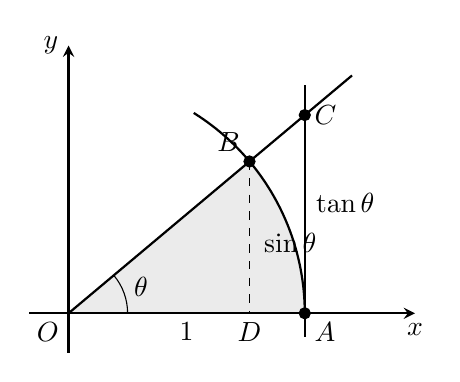
\begin{tikzpicture}[scale=1.0,>=stealth]
  \fill[black!8] (0,0) -- (3,0) arc[start angle=0,end angle=40,radius=3] -- cycle;
  \draw[thick,->] (-0.5,0) -- (4.4,0) node[below] {$x$};
  \draw[thick,->] (0,-0.5) -- (0,3.4) node[left] {$y$};
  \draw[thick] (3,0) arc[start angle=0,end angle=58,radius=3];
  \draw[thick] (0,0) -- (3.6,3.02);
  \draw[thick] (3,-0.3) -- (3,2.9);
  \draw[dashed] (2.298,1.928) -- (2.298,0);
  \draw[fill] (2.298,1.928) circle (2pt) node[above left] {$B$};
  \draw[fill] (3,0) circle (2pt) node[below right] {$A$};
  \draw[fill] (3,2.517) circle (2pt) node[right] {$C$};
  \node[below left] at (0,0) {$O$};
  \node[below] at (2.298,0) {$D$};
  \node[right] at (2.36,0.9) {$\sin\theta$};
  \node[right] at (3.02,1.4) {$\tan\theta$};
  \draw[thin] (0.75,0) arc[start angle=0,end angle=40,radius=0.75];
  \node at (20:0.98) {$\theta$};
  \node[below] at (1.5,0) {$1$};
\end{tikzpicture}
\end{center}

একক বৃত্তে $OA = OB = 1$ এবং $\angle AOB = \theta$, যেখানে
$0 < \theta < \tfrac{\pi}{2}$। $B$ থেকে $OA$-এর উপর লম্ব $BD$, তাই
$BD = \sin\theta$। $A$ বিন্দুতে বৃত্তের স্পর্শক টানলে সে $OB$-এর বর্ধিতাংশকে
$C$ বিন্দুতে ছেদ করে, এবং সমকোণী ত্রিভুজ $OAC$ থেকে $AC = \tan\theta$।

এবার তিনটি ক্ষেত্রফল তুলনা করি। ত্রিভুজ $OAB$ পুরোপুরি sector $OAB$-এর ভেতরে,
আর sector-টি পুরোপুরি ত্রিভুজ $OAC$-এর ভেতরে। Sector-এর ক্ষেত্রফল হলো পূর্ণ
বৃত্তের $\dfrac{\theta}{2\pi}$ অংশ, অর্থাৎ
$\dfrac{\theta}{2\pi} \cdot \pi \cdot 1^{2} = \dfrac{\theta}{2}$। সুতরাং
\[
  \underbrace{\tfrac{1}{2}\sin\theta}_{\triangle OAB}
  \;<\; \underbrace{\tfrac{\theta}{2}}_{\mathrm{sector}}
  \;<\; \underbrace{\tfrac{1}{2}\tan\theta}_{\triangle OAC} ,
\]
অর্থাৎ
\[
  \sin\theta < \theta < \tan\theta .
\]
এই একটি অসমতাই সব বলে দেয়। $\sin\theta$ দিয়ে ভাগ করে ($\sin\theta > 0$, তাই
চিহ্ন বদলায় না) পাই $1 < \dfrac{\theta}{\sin\theta} < \dfrac{1}{\cos\theta}$,
অর্থাৎ
\[
  \cos\theta < \frac{\sin\theta}{\theta} < 1 .
\]
$\theta$ ছোট হলে $\cos\theta$ প্রায় $1$, তাই $\dfrac{\sin\theta}{\theta}$
দুই পাশ থেকে চাপা পড়ে $1$-এর দিকে যায়। এখান থেকেই $\sin\theta \approx \theta$।

কতটুকু ভুল হচ্ছে, সেটাও একই অসমতা থেকে মাপা যায়। উপরের সম্পর্ক থেকে
$\theta - \sin\theta < \theta(1-\cos\theta)$, আর অর্ধ কোণের সূত্র বলছে
$1 - \cos\theta = 2\sin^{2}\dfrac{\theta}{2} < 2\left( \dfrac{\theta}{2}
\right)^{2} = \dfrac{\theta^{2}}{2}$ (এখানে আবার $\sin x < x$ ব্যবহার করা হলো)।
সুতরাং
\[
  0 < \theta - \sin\theta < \frac{\theta^{3}}{2} .
\]
অর্থাৎ ভুলটা $\theta^{3}$-এর মাপের, যা $\theta$ ছোট হলে ভয়ানক দ্রুত কমে।

$\cos$-এর সূত্রটিও ওই একই লাইন থেকে আসে:
\[
  \cos\theta = 1 - 2\sin^{2}\frac{\theta}{2}
  \approx 1 - 2\left( \frac{\theta}{2} \right)^{2}
  = 1 - \frac{\theta^{2}}{2} .
\]
আর যেহেতু $\sin\dfrac{\theta}{2} < \dfrac{\theta}{2}$, তাই
$1 - \dfrac{\theta^{2}}{2} < \cos\theta < 1$; অর্থাৎ আসন্ন মানটি সত্যিকারের
মানের চেয়ে সামান্য ছোট।

সংখ্যায় দেখা যাক।

\begin{center}
\begin{tabular}{c|c|c|c|c}
 $\theta$ (ডিগ্রি) & $\theta$ (radian) & $\sin\theta$ & $\cos\theta$
 & $1-\theta^{2}/2$ \\ \hline
 $1$  & $0.01745$ & $0.017452$ & $0.999848$ & $0.999848$ \\
 $5$  & $0.08727$ & $0.087156$ & $0.996195$ & $0.996192$ \\
 $10$ & $0.17453$ & $0.173648$ & $0.984808$ & $0.984769$ \\
 $20$ & $0.34907$ & $0.342020$ & $0.939693$ & $0.939077$ \\
\end{tabular}
\end{center}

\begin{remark}
$\cos\theta \approx 1$ লিখলেই তো হতো, দ্বিতীয় পদটা কেন দরকার? কারণ অনেক ভৌত
রাশিতে $1$ পদটি কাটাকাটি যায় এবং যা টিকে থাকে সেটাই উত্তর। যেমন $L$ দৈর্ঘ্যের
দোলকের ববটি $\theta$ কোণে ঝুললে সে কতটুকু উপরে ওঠে? উচ্চতা
$h = L - L\cos\theta = L(1-\cos\theta)$। এখানে $\cos\theta \approx 1$ বসালে
$h = 0$ পাওয়া যেত, যা অর্থহীন; কিন্তু $\cos\theta \approx 1 -
\tfrac{\theta^{2}}{2}$ বসালে $h \approx \dfrac{L\theta^{2}}{2}$, আর সেখান থেকেই
দোলকের স্থিতিশক্তি ও পর্যায়কাল বেরিয়ে আসে। কোন পদ পর্যন্ত রাখতে হবে তা নির্ভর
করে কী কাটাকাটি যাচ্ছে তার উপর।
\end{remark}

\begin{remark}
এখানে ``যত ছোট, তত ভালো'' কথাটা যে অর্থে ব্যবহার হচ্ছে তার নিখুঁত রূপ হলো
$\lim_{\theta \to 0} \dfrac{\sin\theta}{\theta} = 1$, যা ১৪ নম্বর অধ্যায়ে
সংজ্ঞাসহ আসবে; উপরের অসমতাটিই সেখানে প্রমাণের মূল হাতিয়ার হবে। আর ১৫ নম্বর
অধ্যায়ে Taylor series হাতে এলে দেখা যাবে
\[
  \sin\theta = \theta - \frac{\theta^{3}}{6} + \cdots, \qquad
  \cos\theta = 1 - \frac{\theta^{2}}{2} + \frac{\theta^{4}}{24} - \cdots ,
\]
অর্থাৎ এই অনুচ্ছেদের সূত্র দুটি আসলে ওই অসীম ধারার প্রথম কয়েকটি পদ, আর
বাদ দেওয়া পদগুলো কত বড় তাও তখন হিসাব করা যাবে।
\end{remark}

\begin{example}
$\theta = 6^{\circ}$-এর জন্য $\sin\theta$ ও $\cos\theta$ ছোট কোণের সূত্র দিয়ে
বের করো এবং প্রকৃত মানের সঙ্গে তুলনা করো।
\end{example}

\begin{solbox}
প্রথমে radian-এ বদলাই: $6^{\circ} = 6 \times \dfrac{\pi}{180} = 0.104720$।

আসন্ন মান: $\sin\theta \approx 0.104720$ এবং
\[
  \cos\theta \approx 1 - \frac{(0.104720)^{2}}{2} = 1 - 0.005483 = 0.994517 .
\]
প্রকৃত মান: $\sin 6^{\circ} = 0.104528$ এবং $\cos 6^{\circ} = 0.994522$।

আপেক্ষিক ভুল: sine-এর ক্ষেত্রে
$\dfrac{0.104720-0.104528}{0.104528} \approx 0.18\%$, আর cosine-এর ক্ষেত্রে
প্রায় $0.0005\%$। উপরের সীমা মিলিয়ে দেখো: $\theta^{3}/2 = 0.00057$, আর
প্রকৃত পার্থক্য $0.000192$, সত্যিই সীমার ভেতরে।
\end{solbox}

\prob{2} $\theta = 2^{\circ}$-এর জন্য ছোট কোণের সূত্রে $\sin\theta$ ও
$\cos\theta$ নির্ণয় করো, এবং $\theta - \sin\theta < \theta^{3}/2$ সীমাটি
যাচাই করো। (প্রকৃত মান: $\sin 2^{\circ} = 0.0348995$,
$\cos 2^{\circ} = 0.9993908$।)

\begin{sol}
$2^{\circ} = 0.0349066$ radian।

আসন্ন মান $\sin\theta \approx 0.0349066$, প্রকৃত $0.0348995$; পার্থক্য
$0.0000071$, অর্থাৎ আপেক্ষিক ভুল প্রায় $0.02\%$।

$\cos\theta \approx 1 - \dfrac{(0.0349066)^{2}}{2} = 1 - 0.00060924
= 0.99939076$, প্রকৃত $0.9993908$; পার্থক্য প্রায় $4 \times 10^{-8}$।

সীমা যাচাই: $\dfrac{\theta^{3}}{2} = \dfrac{(0.0349066)^{3}}{2}
\approx 2.13 \times 10^{-5}$, আর প্রকৃত পার্থক্য
$7.1 \times 10^{-6}$, যা সত্যিই ছোট। সীমাটি ঢিলে, কিন্তু সঠিক।
\end{sol}

\prob{3} $L$ দৈর্ঘ্যের সুতোয় ঝোলানো $m$ ভরের একটি দোলক উল্লম্ব থেকে $\theta$
কোণে আছে। সুতো বরাবর ছাড়া বাকি দিকে (অর্থাৎ গতির দিকে) মাধ্যাকর্ষণের উপাংশ
$mg\sin\theta$, আর ববটির অনুভূমিক সরণ প্রায় $x = L\sin\theta$।
\begin{enumerate}
  \item দেখাও যে $\theta$ ছোট হলে পুনরুদ্ধারী বল প্রায় $-\dfrac{mg}{L}x$,
        অর্থাৎ সরণের সমানুপাতিক।
  \item $\theta = 10^{\circ}$-এ $\sin\theta$-কে $\theta$ দিয়ে বদলালে কত
        শতাংশ ভুল হয়?
\end{enumerate}

\begin{sol}
\begin{enumerate}
  \item ছোট $\theta$-এর জন্য $\sin\theta \approx \theta$, তাই
        $x \approx L\theta$, অর্থাৎ $\theta \approx x/L$। বলটি সরণের বিপরীত
        দিকে কাজ করে, তাই
        \[
          F = -mg\sin\theta \approx -mg\theta \approx -\frac{mg}{L}x .
        \]
        অর্থাৎ বল সরণের সমানুপাতিক এবং বিপরীতমুখী, যা সরল দোলগতির (simple
        harmonic motion) শর্ত। ছোট কোণের আসন্নীকরণ না করলে $\sin\theta$
        পদটি থেকে যেত এবং সমীকরণটি আর সরল থাকত না।
  \item $10^{\circ} = 0.174533$ radian এবং $\sin 10^{\circ} = 0.173648$।
        আপেক্ষিক ভুল
        \[
          \frac{0.174533 - 0.173648}{0.173648} \approx 0.0051 ,
        \]
        অর্থাৎ প্রায় $0.51$ শতাংশ। এই কারণেই পরীক্ষাগারে দোলক নিয়ে কাজ করার
        সময় বলা হয় বিস্তার ছোট রাখতে; $10^{\circ}$ পর্যন্ত ভুল এক শতাংশেরও কম।
\end{enumerate}
\end{sol}

\prob{3} ২ সেন্টিমিটার ব্যাসের একটি মুদ্রা চোখ থেকে ৬০ সেন্টিমিটার দূরে ধরা
হলো।
\begin{enumerate}
  \item মুদ্রাটি কত কোণ জুড়ে আছে? radian ও ডিগ্রি দুটিতেই লেখো।
  \item চাঁদের কৌণিক ব্যাস প্রায় $0.0093$ radian। মুদ্রাটি চাঁদের কত গুণ বড়
        দেখাচ্ছে?
\end{enumerate}

\begin{sol}
\begin{enumerate}
  \item বস্তুটি দূরত্বের তুলনায় ছোট, তাই তার কৌণিক ব্যাস প্রায় ব্যাসকে
        দূরত্ব দিয়ে ভাগ করলে যা হয় তাই; কারণ
        $\tan(\theta/2) = \dfrac{1}{60}$ এবং ছোট কোণে $\tan$ ও কোণ প্রায় সমান।
        সুতরাং
        \[
          \theta \approx \frac{2}{60} = 0.0333 \ \mathrm{radian}
          = 0.0333 \times \frac{180}{\pi} \approx 1.91^{\circ} .
        \]
  \item $\dfrac{0.0333}{0.0093} \approx 3.6$, অর্থাৎ মুদ্রাটি চাঁদের প্রায়
        সাড়ে তিন গুণ বড় দেখাচ্ছে।
\end{enumerate}
লক্ষ করো, এখানে ``কত বড় দেখাচ্ছে'' মানে কৌণিক ব্যাস, প্রকৃত আকার নয়; ১১ নম্বর
অধ্যায়ের solid angle ছিল এই ধারণারই ত্রিমাত্রিক সম্প্রসারণ।
\end{sol}

\end{document}
